\newchapter{Einleitung}
\label{kap:1}


Partielle Differentialgleichungen sind in vielen Bereichen der Natur- und Ingenieurswissenschaften wiederzufinden. Da die exakte Lösung nicht immer existiert, bzw. die Bestimmung solch einer Lösung beliebig kompliziert werden kann, haben numerische Löser für partielle Differnetialgleichungen in den letzen Jahrzehnten immer mehr an Bedeutung gewonnen. Insbesondere ist dies durch die Weiterentwicklung der Computertechnologie und verfügbaren Rechenleistung begründet. Die Lösung kann daher z.B. mittels \idx{Galerkin-Verfahren} (bzw. Finiter-Elemente-Methode\index{Finite-Elemente-Methode}) ermittelt werden. Hierbei wird die eigentliche Differentialgleichung nur noch approximativ auf einem Gitter gelöst, wobei wir durch Verfeinerung des Gitters die Genauigkeit der Lösung erhöhen, was allerdings auch zu höherem Rechenaufwand führt. Daher ist es sinnvoll, die Verfeinerung des Gitters gerade so zu steuern, dass möglichst wenig, aber für eine hinreichend genaue Lösung noch genügend Elemente verfeinert werden. Diese Verfahren werden als \textit{\idx{adaptive Verfeinerungsstategie}n} bezeichnet und sind im Allgemeinen von der Form:
\[
	\text{solve}\ \ \ra \ \ \text{estimate}\ \ \ra\ \ \text{mark}\ \ \ra\  \ \text{refine} \, .
\]
Da die exakte Lösung in den meisten Fällen nicht bekannt ist, ist der Schritt "`estimate"' von entscheidender Bedeutung. Hierbei wird der Fehler zur exakten Lösung auf dem nächsten Gitter mittels eines a posteriori Fehlerschätzer bzgl. des aktuellen Gitters abgeschätzt, was Zuverlässigkeit und Effizienz des Schätzers voraussetzt. Dadurch wird sichergestellt, dass durch Verringerung des Fehlerschätzers auch  der exakte Fehler kleiner wird. 

Es gibt fünf Klassen von a posteriori Fehlerschätzern (vgl. \cite{BraeFEM}):
\begin{itemize}
\item Residuale Schätzer,
\item Schätzer über ein lokales Neumann-Problem,
\item Schätzer über ein lokales Dirichlet-Problem,
\item Schätzer durch Mittelung,
\item Hierarchische Schätzer.
\end{itemize}
Die in der Literatur  am häufigsten verwendete Klasse sind die residualen a posteriori Fehlerschätzer (vgl. bspw. \cite{BraeFEM}, \cite{BraeLook}, \cite{BraeCar}, \cite{BraeCar2}, \cite{MorNoc}). In der vorliegenden Arbeit wollen wir einen hierarchischen Fehlerschätzer untersuchen. Solche Schätzer basieren auf einer Hierarchie von Ansatzräumen, d.h. man untersucht das gegebene Problem in einem "`besseren"' Finite-Element-Raum und schätzt damit den Fehler bzgl. der "`schlechteren"' \idx{Galerkin-Approximation} ab. Der dadurch entstehende  Fehlerschätzer  wird dann in lokale Anteile bzgl. der Elemente des Gitters aufgeteilt. Damit können im Schritt "`mark"'  genau diejenigen Elemente ausgewählt werden, die an dem berechneten Schätzer einen hohen lokalen Anteil haben., d.h. verfeinere diejenigen Elemente $T$, für die
\[
	\sum_{T} \eta_T \ge \theta\, \eta 
\]
gilt, wobei $\eta_T$ die lokalen Anteile des Schätzers $\eta$ darstellen und $\theta \in (0,1)$ ein gegebener Parameter ist, der ein Verhältnis der zu verfeinernden Elemente angibt.

Diese Verfeinerungsstrategie wollen wir in der vorliegenden Arbeit zu-nächst für ein Hindernisproblem untersuchen. Ein Modellproblem eines Hindernisproblems stellt z.B. eine in einem Gebiet $\Omega$ eingespannte Membran dar, die mit einer Last $f$ vertikal belastet und deren Auslenkung $u: \Omega \ra \R$ durch ein Hindernis $\psi$ behindert wird. Da die in der Membran gespeicherte Energie minimal ist, kann man die Auslenkung dieser durch ein Optimierungsproblem von der Form
\begin{align}\label{eq:1.1}
	u = \arg\min_{v \in K} J(v) = \frac 12 \int_{\Omega} \nabla v \nabla v \, dx - \int_\Omega f v \, dx
\end{align}
modellieren, wobei $K$ die Menge der Auslenkungen $u$ ist, die oberhalb des Hindernisses $\psi$ liegen, d.h. $u\ge \psi$ erfüllen.  In Abbildung \ref{abb:1.1} sind im Vergleich die Auslenkungen einer auf einem Kreisgebiet belasteten Membran ohne und mit (ebenem) Hindernis dargestellt. Für das Problem \eqref{eq:1.1} werden wir in Kapitel \ref{kap:4.1} einen wie oben beschriebenen hierarchischen a posteriori Fehlerschätzer herleiten, wobei wir die lokale Aufteilung des Schätzers bzgl. der Knoten, nicht der Elemente $T$, des verwendeten Gitters untersuchen werden. Das Hauptresultat dieser Arbeit befindet sich in Theorem \ref{theorem:4.22}, welches  die Verwendung des Schätzers ermöglicht. In diesem Hauptresultat werden wir zeigen, dass der betrachtete a posteriori Fehlerschätzer eine obere Schranke für den exakten Fehler $J(u_{\mcal S}) - J(u)$ im Energiefunktional $J$ aus \eqref{eq:1.1} bis auf Terme höherer Ordnung (Oszillationsterme) darstellt.

\begin{figure}[h]
\begin{center}
\subfigure[ohne Hindernis]{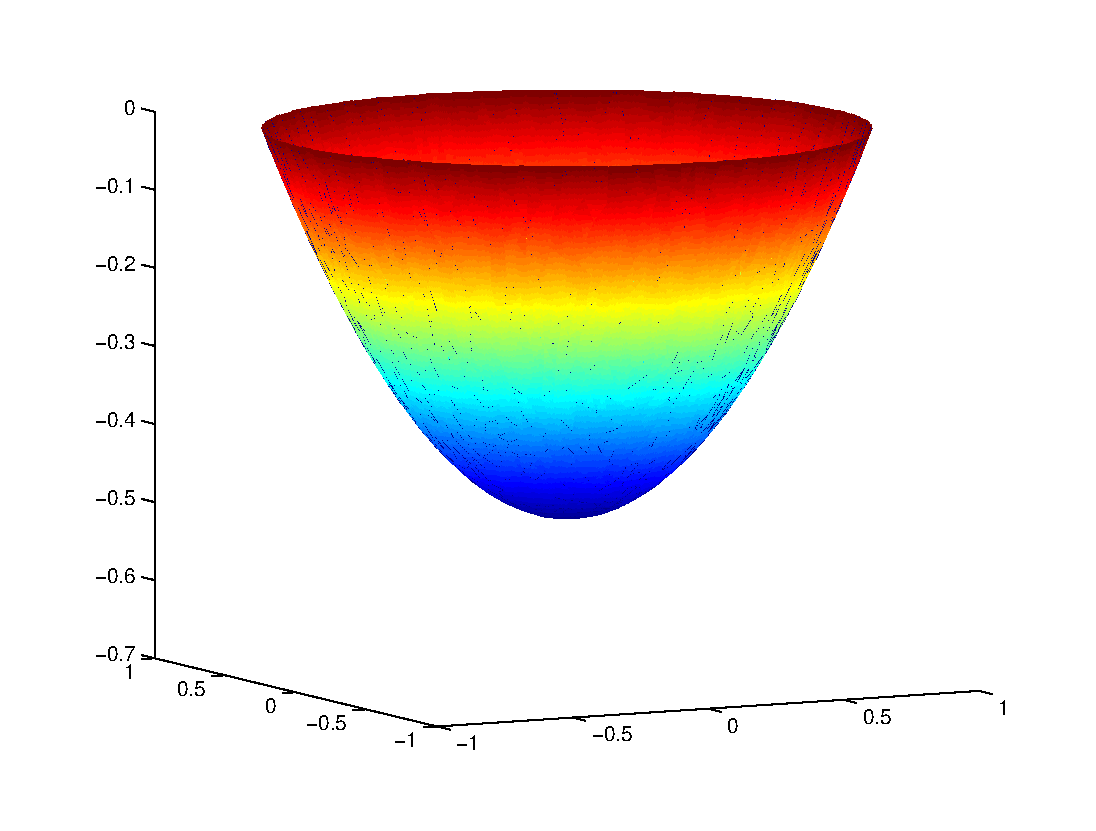
\includegraphics[width=6.25cm]{Abbildungen/bsp_ohne_hindernis.eps}}
\hfill
\subfigure[mit Hindernis: Ebene $z=-0,28$]{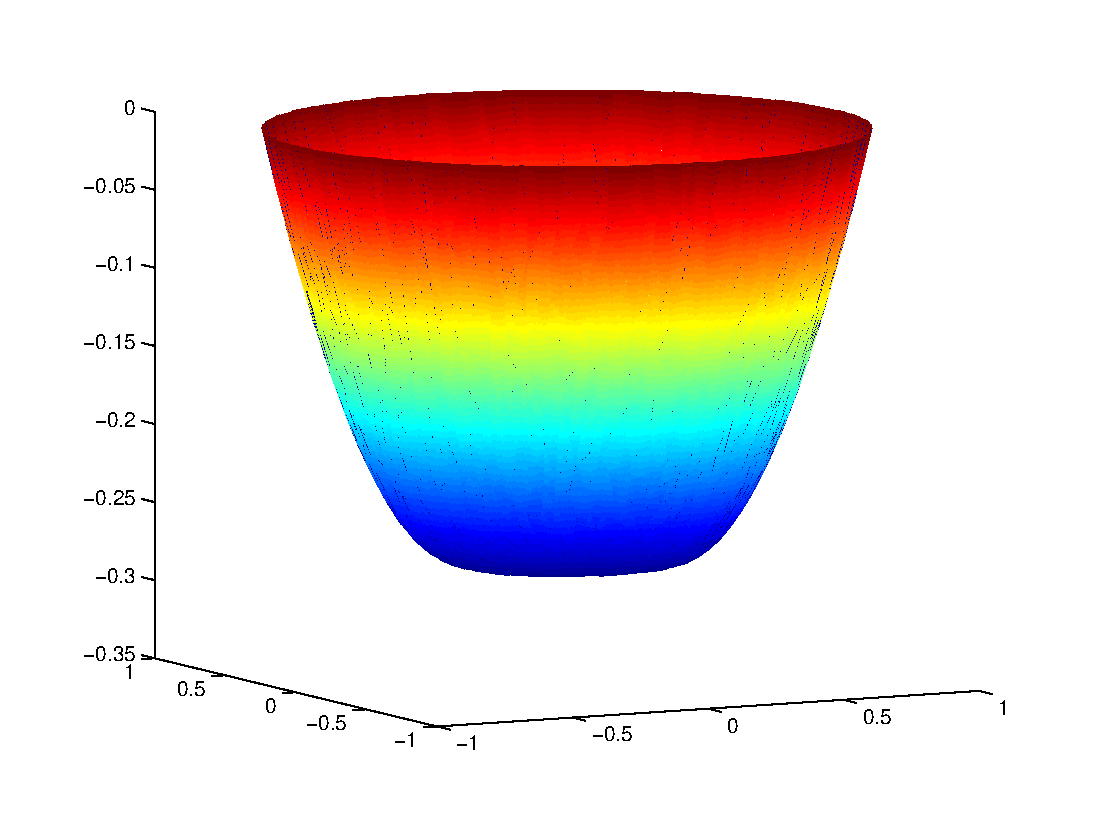
\includegraphics[width=6.25cm]{Abbildungen/bsp_mit_hindernis.eps}}
\end{center}
\caption{Auslenkung einer eingespannten Membran unter Einwirkung einer vertikalen Lastfunktion $f$\label{abb:1.1}}
\end{figure}


Nachdem wir in Kapitel \ref{kap:4} einen hierarchischen a posteriori Fehlerschätzer für das Modellproblem \eqref{eq:1.1} untersucht haben, wollen wir diesen auf Kontaktprobleme übertragen. Für residuale a posteriori Fehlerschätzer sind diese bereits in der Literatur (vgl. z.B. \cite{CarWri}, \cite{WriggersContact} und \cite{HanJoh}) vielfältig untersucht worden. Daher wollen wir ein Kontaktproblem für den in dieser Arbeit eingeführten hierarchischen Fehlerschätzer untersuchen.

Kontaktprobleme sind Probleme aus der Strukturmechanik und stellen eine Anwendung von partiellen Differentialgleichungen unter Nebenbedingung (nämlich der Kontaktbedingung) dar. Wir werden uns in dieser Arbeit mit einem vereinfachten Kontaktproblem, dem \textit{\idx{Signorini-Kontakt}problem} beschäftigen, d.h. es gibt keine Reibungskräfte auf der Kontaktfläche. Außerdem werden wir von einem linear elastischen Fall ausgehen, d.h. das Hooke'sche Gesetz gilt. Die Lösung eines Kontaktproblems kann wie oben eindeutig (vgl. Kapitel \ref{kap:3.2}) durch die Minimierung des Energiefunktionals
\begin{align}\label{eq:1.2}
	\mcal J (\bs v) = \frac 12 \int_\Omega \bs \sigma (\bs v):\bs \eps(\bs v) \, d\Omega - \int_\Omega \bs b\cdot \bs v \, d\Omega - \int_{\Gamma} \bs t\cdot \bs v \, d\Gamma 
\end{align}
über $\mscr K$ berechnet werden, wobei die Menge $\mscr K$ diejenigen Verschiebungsfelder $\bs v$ enthält, die die Kontaktbedingung $\bs v \cdot\bs n - g \le 0$ erfüllen. Die Funktion $g$ gibt hierbei die Lücke zwischen den beiden Körpern an und wird daher auch als \textit{\idx{Gap-Funktion}} bezeichnet. Diese  stellt für Problem \eqref{eq:1.2} also das Hindernis dar, wie zuvor $\psi$ für \eqref{eq:1.1}. In Kapitel \ref{kap:4.4} werden dann die Übertragungen der Konzepte des Fehlerschätzers für Problem \eqref{eq:1.1} beschrieben. Weiter stellt $\bs \sigma$ die Spannung, $\bs \eps$ die Verzerrung und $\bs b$ die Volumenlast (z.B. Gewichtskraft) im vorliegenden Körper dar, der durch $\Omega$ beschriebenen wird. Die Funktion $\bs t$ beschreibt eine Oberflächenlast, die auf den Körper wirkt.

Zunächst werden wir jedoch in Kapitel \ref{kap:3} zeigen, dass die beiden Probleme \eqref{eq:1.1} und \eqref{eq:1.2} grundlegend auf dieselben Variationsungleichungen führen und die Existenz einer eindeutigen Lösung für solch eine Variationsungleichung, und damit auch für die jeweiligen Probleme, zeigen.

Zuvor werden in Kapitel \ref{kap:2}  grundlegende Konzepte zu Hilberträumen, Variationsrechnung, adaptive Verfeinerungsstrategien und der Strukturmechanik eingeführt. Weitere Resultate, die in der vorliegenden Arbeit verwendet werden und nicht in Kapitel \ref{kap:2} aufgeführt sind, können in Anhang \ref{anhang:A} (Funktionalanalysis), \ref{anhang:B} (Optimierung) und \ref{anhang:C} (Tensorrechnung) nachgeschlagen werden.

Die Lösungsverfahren für die adaptive Verfeinerung der Hindernis- bzw. Kontaktprobleme werden in Matlab implementiert und die wichtigsten Vorgehensweisen hierfür in Kapitel \ref{kap:5} beschrieben. Der Quellcode ist im Detail im Anhang \ref{anhang:D} einzusehen.

In Kapitel \ref{kap:6} werden wir abschließend mehrere Beispiele für Hindernis- bzw. Kontaktprobleme präsentieren, welche die Resultate aus Kapitel \ref{kap:4} untermauern.



\newpage

%%% Local Variables: 
%%% mode: latex
%%% TeX-master: "Skript"
%%% End: 
